%----------------------------------------------------------------------------------------
%	PACKAGES AND THEMES
%----------------------------------------------------------------------------------------
\documentclass[aspectratio=169,xcolor=dvipsnames]{beamer}
\usetheme{Simple}

\usepackage{hyperref}
\usepackage{graphicx} % Allows including images
\usepackage{booktabs} % Allows the use of \toprule, \midrule and \bottomrule in tables
\usepackage{tikz}
\usepackage{changepage}
\tikzset{process/.style={draw=black}}
\tikzset{machine/.style={minimum width=5.3cm,minimum height=1.9cm,draw=black,densely dashed}}
\tikzset{doublearrow/.style={<->,>=latex}}
\usetikzlibrary{arrows.meta, positioning}


%----------------------------------------------------------------------------------------
%	TITLE PAGE
%----------------------------------------------------------------------------------------

% The title
\title[short title]{Exp3}
\subtitle{Seminar Advanced Topics in Reinforcement Learning and Decision Making }

\author[Kuba] {Jakub Tłuczek \\ \texttt{jakub.tluczek@unine.ch}}

\institute[UniNE] % Your institution may be shorthand to save space
{
    % Your institution for the title page
    Universite de Neuchâtel\\
    Swiss Joint Master in Computer Science
    \vskip 3pt
}

\titlegraphic{
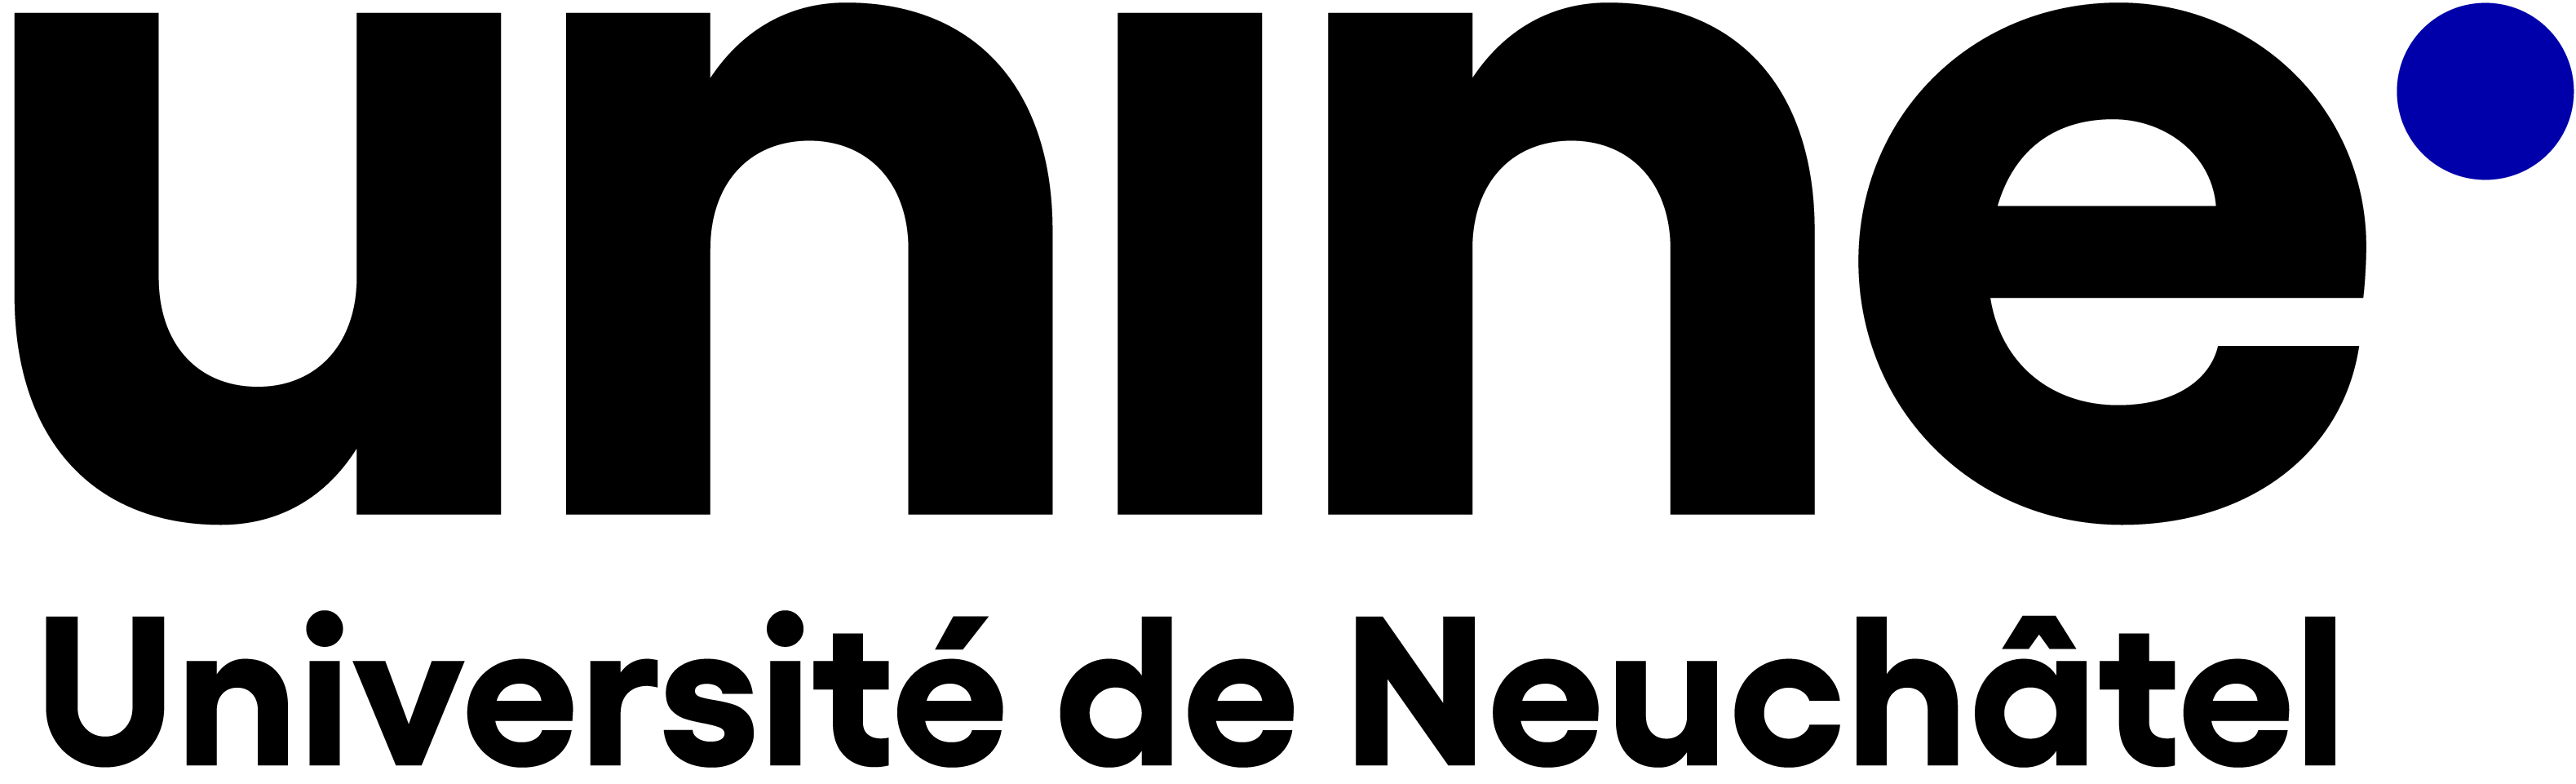
\includegraphics[width=3cm]{unine_logo_couleur.png}
\hspace{5cm}

\includegraphics[width=3cm]{jmcs.png}
}
\date{\today} % Date, can be changed to a custom date


%----------------------------------------------------------------------------------------
%	PRESENTATION SLIDES
%----------------------------------------------------------------------------------------

\begin{document}

\begin{frame}
    % Print the title page as the first slide
    \titlepage
\end{frame}

\begin{frame}{Overview}
    % Throughout your presentation, if you choose to use \section{} and \subsection{} commands, these will automatically be printed on this slide as an overview of your presentation
    \tableofcontents
\end{frame}

\section{Adversarial Bandits}
\begin{frame}{Adversarial Bandits}
  \begin{itemize}
  \item Reward sequence $(x_t)_{t=1}^n$, with $x_{t,i}$ reward of arm $i$ at time $t$, \alert{fixed by an adversary}.
  \item Agent's action is drawn from a distribution $P_t \in \mathcal{P}_{k-1}$, where $\mathcal{P}_d$ is a probability simplex over $d+1$ actions (i.e. $\mathcal{P}_d = \{ p \in [0,1]^{d+1} : ||p||_1 = 1 \} = \{ p \in [0,1]^{d+1} : \sum_i p_i = 1 \}$. 
  \item The policy $\pi$ maps from  histories onto the distribution over action
    \[
      \pi\; : \; ([k] \times [0,1])^{*} \rightarrow \mathcal{P}_{k-1}.
    \]
  \item  At each timestep $t$:
    \begin{enumerate}
    \item Agent chooses distribution $P_t$
    \item Action is drawn $A_t \sim P_t$
    \item Reward $X_t = x_{t A_t}$ is observed.
    \end{enumerate}
  \end{itemize}
\end{frame}

\begin{frame}{Adversarial Bandits regret}

    Regret in case of an adversarial bandit can be summarized as:

    \begin{equation}
        R_n(\pi, x) = \max_{i \in [k]} \sum_{t=1}^n x_{ti} - \mathbb{E}\left[ \sum_{t=1}^n x_{t A_t}\right]
    \end{equation}

    While Worst case regret for some policy $\pi$ is:

    \begin{equation}
        R^{*}_n(\pi) = \sup_{x \in [0,1]^{n \times k}} R_n(\pi, x)
    \end{equation}
\end{frame}


\section{Importance weighted estimators}
\begin{frame}{Importance weighted estimators}
    Before we go into the Exp3 algorithm, we have to introduce an unbiased estimator for reward $\hat{X_{ti}}$ at time $t$ for arm $i$. It is defined as:

    \begin{equation}
        \hat{X}_{ti} = \frac{\mathbb{I}\{A_t = i\}X_t}{P_{ti}}
    \end{equation}

    where $P_{ti}$ is the probability of selecting arm $i$ at time $t$. Why is $\hat{X_{ti}}$ unbiased?

    \begin{equation}
        \mathbb{E}\left[ \hat{X}_{ti} \right] = \mathbb{E} \left[ \frac{\mathbb{I}\{A_t = i\}X_t}{P_{ti}} \right] = \sum_j P_{tj} \hat{X}_{ti} = P_{ti} \hat{X}_{ti} + \sum_{j \neq i} P_{tj} \cdot 0 = P_{ti} \frac{X_t}{P_{ti}} = x_{ti}
    \end{equation}
\end{frame}

\begin{frame}{Loss-based importance weighted estimator}
    Another unbiased estimator would be:

    \begin{equation}
        \hat{X}_{ti} = 1 - \frac{\mathbb{I}\{A_t = i\}(1 - X_t)}{P_{ti}} 
    \end{equation}

    where we can prove it is unbiased by substituting $Y_t = 1 - X_t$. The advantage of loss based estimator is, that while in the case of estimator from previous slide its variance is:

    \begin{equation}
        \mathbb{V}\left[ \frac{\mathbb{I}\{A_t = i\}X_t}{P_{ti}} \right] = x^2_{ti} \frac{1-P_{ti}}{P_{ti}}
    \end{equation}

    while loss based estimator's variance is proportional to $(1 - x_{ti})^2$:

    \begin{equation}
        \mathbb{V}\left[ 1 - \frac{\mathbb{I}\{A_t = i\}(1 - X_t)}{P_{ti}}  \right] = (1 - x_{ti})^2 \frac{1-P_{ti}}{P_{ti}}
    \end{equation}
\end{frame}

\section{Exp3}
\begin{frame}{Exp3}
    \textbf{Exp}onential-weight algorithm for \textbf{exp}loration and \textbf{exp}loitation (hence \textbf{Exp}3) is based on changing the probabilities for each actions based on term $\hat{S}_ti = \sum_{s=1}^{t} \hat{X}_si$, which is the sum of estimated rewards up until current round $t$.

    Probability for each arm at each timestep is calculated using the following, softmax-like, formula:

    \begin{equation}
        P_{ti} = \frac{\exp(\eta \hat{S}_{t-1, i})}{\sum_{j} \exp(\eta \hat{S}_{t-1, j})}
    \end{equation}

    Then, $A_t \sim P_t$ is played, reward $X_t$ observed and estimated rewards adjusted:

    \begin{equation}
        \hat{S}_{ti} = \hat{S}_{t-1, i} + 1 - \frac{\mathbb{I}\{ A_t = i \}(1 - X_t)}{P_{ti}}
    \end{equation}
\end{frame}

\begin{frame}{Exp3 expected regret}
    Regret for Exp3 is bounded from above by:

    \begin{equation}
        R_n \leq \frac{\log (k)}{\eta} + \eta nk
    \end{equation}

    when we set learning rate $\eta = \sqrt{\log(k)/nk}$, then the regret bound would be optimized as follows:

    \begin{equation}
        R_n \leq 2 \sqrt{nk \log(k)}
    \end{equation}
\end{frame}

\subsection{Proof outline}
\begin{frame}
  Define
  \[ 
    \hat{S}_n = \sum_{t, i} P_{ti} \hat{X}_{t,i},
    \qquad
    W_t = \sum_{j=1}^k \exp\left(\eta \hat{S}_{t,j}\right)
  \]
  \pause
  We now bound the exponential term
  \[
    \exp(\eta \hat{S}_{ni} \leq \sum_{j=1}^k 
  \]
\end{frame}

\section{Adversarial linear bandits}
\begin{frame}{Adversarial linear bandits}
    In adversarial linear settings, actions from action set $\mathbf{\mathcal{A}} \subset \mathbb{R}^d$ are $d$-dimensional vectors, just as reward $x_t$ at time $t$. Reward in this setting is given by inner product $\langle A_t, x_t \rangle$. Without loss of generality, we can switch to losses $y_t = 1 - x_t$. Therefore, if observed loss would be defined as $Y_t = \langle A_t, y_t \rangle$, then regret after $n$ steps is defined as:

    \begin{equation}
        R_n = \mathbb{E} \left[ \sum_{t=1}^{n} Y_t \right] - \min_{a \in \mathbf{\mathcal{A}}} \sum_{t=1}^{n} \langle a, y_t \rangle
    \end{equation}
\end{frame}

\section{Exp3 for adversarial linear bandits}
\begin{frame}{Exp3 for finite exponential weights}
    Probability distribution $P_t(a)$ is given by mixture distribution:

    \begin{equation}
        P_t(a) = (1 - \gamma)\tilde{P}_t(a) + \gamma \pi(a)
    \end{equation}

    where $\pi(a)$ is an exploration distribution mapping simplex $\mathbf{\mathcal{A}} \rightarrow [0,1] ; \sum_{a \in \mathbf{\mathcal{A}}} \pi(a) = 1$, while $\tilde{P}_t(a)$ is a probability mass function:

    \begin{equation}
        \tilde{P}_t(a) \propto \exp \left( -\eta \sum_{s=1}^{t-1} \hat{Y}_s(a) \right)
    \end{equation}

    Finally, loss estimate is estimated by $\hat{Y}_t = Q_t^{-1} A_t Y_t$, where $Q_t$ is given by:

    \begin{equation}
        Q_t = \sum_{a \in \mathbf{\mathcal{A}}} P_t(a)aa^{\intercal}
    \end{equation}

\end{frame}

\begin{frame}{Exp3 for finite exponential weights}
    Distribution is calculated at each step by:

    \begin{equation}
        P_t(a) = \gamma \pi(a) + (1 - \gamma) \frac{\exp \left( - \eta \sum_{s=1}^{t-1} \hat{Y}_s(a) \right)}{\sum_{a' \in \mathbf{\mathcal{A}}} \exp \left( - \eta \sum_{s=1}^{t-1} \hat{Y}_s(a') \right)}
    \end{equation}

    Action $A_t \sim P_t$ is sampled, loss $Y_t = \langle A_t, y_t \rangle$ is observed and loss estimate is updated using:

    \begin{equation}
        \hat{Y}_t = Q_t^{-1} A_t Y_t
    \end{equation}

\end{frame}

\begin{frame}{Exp3 regret for adversarial linear bandits}
    Exp3 regret is bounded from above by:

    \begin{equation}
        R_n \leq 2 \sqrt{(2g(\pi) + d)n \log(k)}
    \end{equation}

    where $d$ is the dimension of $\mathbf{\mathcal{A}}$, $k$ is the number of arms and $g(\pi)$ equals:

    \begin{equation}
        g(\pi) = max_{a \in \mathbf{\mathcal{A}}} ||a||^2_{Q^{-1}(\pi)}
    \end{equation}
\end{frame}

\begin{frame}{Exp3 for continuous exponential weights}
    If the number of arms is big, or if it goes to $\infty$, then this algorithm becomes intractable. Instead of computing $P_t$ for every arm, we can switch to continuous exponential weights.
    
    Assuming that $\mathbf{\mathcal{A}}$ is convex, distribution is calculated by:

    \begin{equation}
        P_t(B) = \gamma \pi(B) + (1-\gamma) \frac{\int_B \exp \left( - \eta \sum_{s=1}^{t-1} \hat{Y}_s(a) \right)da}{\int_\mathbf{\mathcal{A}} \exp \left( - \eta \sum_{s=1}^{t-1} \hat{Y}_s(a) \right)da}
    \end{equation}

    Rest of the algorithm is analogous to the Exp3 for finite action sets.
\end{frame}


\end{document}